\documentclass[10pt,a4paper]{article}

% ==============================================================================
% IOT PROJECT: AUTOMATIC NIGHT LIGHT SYSTEM (EXACT SINGLE 1-PAGE DOCUMENT)
% Formatted with wide margins for single-line table cells and high-contrast print.
% Department of Computer Science & Engineering / Information Technology
% ==============================================================================
\usepackage[utf8]{inputenc}
\usepackage[T1]{fontenc}
\usepackage{lmodern}
\usepackage[left=0.6in, right=0.6in, top=0.30in, bottom=0.30in]{geometry}
\usepackage{amsmath,amssymb}
\usepackage{xcolor}
\usepackage{listings}
\usepackage{graphicx}
\usepackage{tikz}
\usetikzlibrary{arrows.meta,positioning}
\usepackage{booktabs}
\usepackage{tabularx}
\usepackage{titlesec}
\usepackage{caption}
\usepackage{microtype}
\usepackage{float}

% Disable all running headers, footers, and page numbers for clean print & paste
\pagestyle{empty}
\setlength{\parindent}{0pt}

% Section Titles Formatting
\titleformat{\section}
  {\normalfont\normalsize\bfseries\raggedright}{\thesection}{0.5em}{}[\titlerule]

\titlespacing*{\section}{0pt}{3.0pt}{1.5pt}

% Code Listing Styling (Strict Monochrome with Enlarged Font for High-Contrast Print)
\lstdefinestyle{bwArduino}{
    language=C++,
    basicstyle=\ttfamily\scriptsize,
    keywordstyle=\bfseries,
    commentstyle=\itshape,
    stringstyle=\ttfamily,
    numbers=left,
    numberstyle=\tiny,
    numbersep=5pt,
    stepnumber=1,
    breaklines=true,
    breakatwhitespace=true,
    frame=single,
    rulecolor=\color{black},
    tabsize=2,
    showstringspaces=false,
    columns=fullflexible,
    keepspaces=true,
    lineskip=-0.35pt,
    aboveskip=1.5pt,
    belowskip=1.5pt
}

\lstdefinestyle{bwTerminal}{
    basicstyle=\ttfamily\scriptsize,
    numbers=none,
    breaklines=true,
    breakatwhitespace=true,
    frame=single,
    rulecolor=\color{black},
    columns=fullflexible,
    keepspaces=true,
    lineskip=0.2pt,
    aboveskip=1.5pt,
    belowskip=1.5pt
}

\captionsetup{font=small,labelfont=bf,skip=2pt}

\begin{document}

% ==============================================================================
% DOCUMENT HEADER
% ==============================================================================
\begin{center}
    {\large\bfseries Project: Automatic Night Light System using LDR \& Arduino UNO}\\[0.05cm]
    {\small\textbf{Ambient Light-Adaptive Luminaire Automation --- Program Source Code \& Experimental Output}}
\end{center}
\vspace{-0.22cm}
\rule{\textwidth}{0.9pt}
\vspace{0.02cm}

% ==============================================================================
% 1. PROGRAM SOURCE CODE
% ==============================================================================
\section*{1. Arduino C++ Source Code}

\begin{lstlisting}[style=bwArduino, title={\textbf{Listing P.1: Production Firmware for Automatic Night Light with Moving-Average Filtering \& Hysteresis.}}]
/* Project Work: Automatic Night Light System (Ambient Light-Adaptive Luminaire)
 * Connections: LDR -> A0 (10k Pull-Down) | 5mm LED -> Pin D9 (220 Ohm Resistor) | Baud: 9600 bps */
const int LDR_PIN = A0;              // Analog input pin for LDR potential divider tap
const int LED_PIN = 9;               // Digital output pin for LED actuator
const int THRESHOLD_DARK  = 400;     // Lower hysteresis boundary (Nightfall -> Turn ON)
const int THRESHOLD_LIGHT = 500;     // Upper hysteresis boundary (Daybreak -> Turn OFF)
const int SAMPLES = 10;              // Rolling average window size
int buffer[SAMPLES]; int bufIdx = 0; long runningSum = 0;
bool ledState = false; unsigned long lastLog = 0;

void setup() {
  pinMode(LED_PIN, OUTPUT); digitalWrite(LED_PIN, LOW); // Initialize luminaire extinguished
  Serial.begin(9600);
  for (int i = 0; i < SAMPLES; i++) {
    buffer[i] = analogRead(LDR_PIN); runningSum += buffer[i]; delay(5);
  }
}

void loop() {
  runningSum -= buffer[bufIdx];
  buffer[bufIdx] = analogRead(LDR_PIN);
  runningSum += buffer[bufIdx];
  bufIdx = (bufIdx + 1) % SAMPLES;

  int filteredADC = runningSum / SAMPLES;
  float nodeV = (filteredADC * 5.0) / 1023.0;

  // Dual-Threshold Schmitt Trigger Hysteresis Comparator
  if (filteredADC <= THRESHOLD_DARK) {
    ledState = true;  digitalWrite(LED_PIN, HIGH);     // Darkness detected: Luminaire ON
  } else if (filteredADC >= THRESHOLD_LIGHT) {
    ledState = false; digitalWrite(LED_PIN, LOW);      // Daylight restored: Luminaire OFF
  }

  // Periodic Telemetry Reporting over UART Serial (Every 500 ms)
  if (millis() - lastLog >= 500) {
    lastLog = millis();
    Serial.print("ADC: "); Serial.print(filteredADC);
    Serial.print(" | V: "); Serial.print(nodeV, 2);
    Serial.print("V | Luminaire: ");
    Serial.println(ledState ? "ACTIVE (ON)" : "INACTIVE (OFF)");
  }
  delay(20);
}
\end{lstlisting}

\vspace{0.04cm}

% ==============================================================================
% 2. EXPERIMENTAL OUTPUT & SERIAL TELEMETRY (SERIAL ORDER: 2.A -> 2.B -> 2.C)
% ==============================================================================
\section*{2. Experimental Output, Serial Monitor Telemetry \& Switching Response}

\noindent
\textbf{A. Sensor Calibration \& Operational State Matrix:}\par\vspace{0.03cm}
{\footnotesize
\setlength{\tabcolsep}{4.5pt}
\renewcommand{\arraystretch}{1.16}
\begin{tabularx}{\textwidth}{|c|p{5.0cm}|c|c|c|>{\raggedright\arraybackslash}X|}
\hline
\textbf{\#} & \textbf{Ambient Lighting Environment} & \textbf{Lux Level} & \textbf{ADC (0--1023)} & \textbf{Node Voltage} & \textbf{Luminaire Indicator Status} \\
\hline
1 & Direct Sunlight / High Torch Beam & $> 1000\,\text{lux}$ & $982$ & $4.80\,\text{V}$ & \textbf{OFF} (Full Daylight Inactive) \\
2 & Laboratory Overhead Illumination & $450\,\text{lux}$ & $839$ & $4.10\,\text{V}$ & \textbf{OFF} (Adequate Ambient Lighting) \\
3 & Ambient Twilight / Dusk Transition & $95\,\text{lux}$ & $536$ & $2.62\,\text{V}$ & \textbf{OFF} (Above Turn-ON Threshold) \\
4 & Threshold Border (Nightfall Entry) & $35\,\text{lux}$ & $358$ & $1.75\,\text{V}$ & \textbf{ON} (Night Light Tripped) \\
5 & Covered Sensor / Pitch Darkness & $2\,\text{lux}$ & $104$ & $0.51\,\text{V}$ & \textbf{ON} (Full Luminaire Activation) \\
\hline
\end{tabularx}
}

\vspace{0.10cm}

\noindent
\textbf{B. Real-Time Serial Monitor Stream (9600 Baud):}\par\vspace{0.03cm}
\begin{lstlisting}[style=bwTerminal]
ADC: 982 | V: 4.80V | Luminaire: INACTIVE (OFF)  [Direct Sunlight Exposure]
ADC: 839 | V: 4.10V | Luminaire: INACTIVE (OFF)  [Standard Laboratory Lighting]
ADC: 536 | V: 2.62V | Luminaire: INACTIVE (OFF)  [Twilight Transition Phase]
ADC: 358 | V: 1.75V | Luminaire: ACTIVE (ON)     [Darkness Detected -> LED ON]
ADC: 104 | V: 0.51V | Luminaire: ACTIVE (ON)     [Pitch Darkness -> Sustained ON]
\end{lstlisting}

\vspace{0.10cm}

\noindent
\textbf{C. Schmitt Trigger Dual-Threshold Hysteresis Transfer Curve:}\par\vspace{0.04cm}
{\centering
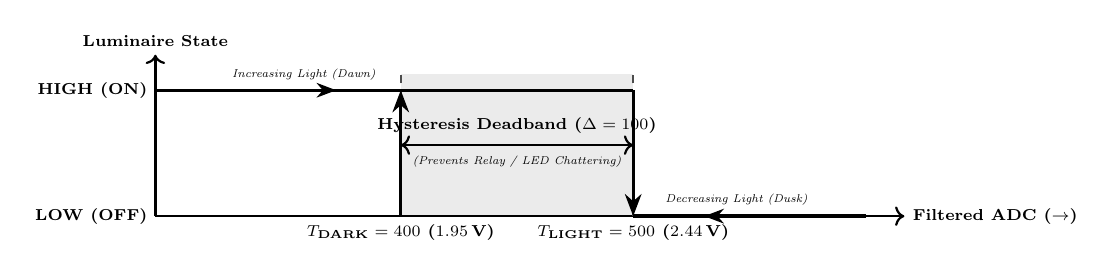
\begin{tikzpicture}[scale=0.82, every node/.style={transform shape}]
    % Shaded deadband region
    \fill[gray!16] (3.8, 0) rectangle (7.4, 2.2);

    % Coordinate Axes
    \draw[->, thick] (0, 0) -- (11.6, 0) node[right, font=\scriptsize\bfseries] {Filtered ADC ($\to$)};
    \draw[->, thick] (0, 0) -- (0, 2.5) node[above, font=\scriptsize\bfseries] {Luminaire State};

    % Threshold vertical dashed lines
    \draw[dashed, thick, black!70] (3.8, 0) -- (3.8, 2.2);
    \node[below, font=\scriptsize\bfseries] at (3.8, 0) {$T_{\text{DARK}} = 400$ ($1.95\,\text{V}$)};

    \draw[dashed, thick, black!70] (7.4, 0) -- (7.4, 2.2);
    \node[below, font=\scriptsize\bfseries] at (7.4, 0) {$T_{\text{LIGHT}} = 500$ ($2.44\,\text{V}$)};

    % Deadband annotation
    \draw[<->, thick] (3.8, 1.1) -- (7.4, 1.1);
    \node[above, font=\scriptsize\bfseries] at (5.6, 1.15) {Hysteresis Deadband ($\Delta = 100$)};
    \node[below, font=\tiny\itshape] at (5.6, 1.05) {(Prevents Relay / LED Chattering)};

    % Upper Branch (HIGH / ON: y = 1.95)
    \draw[very thick] (0, 1.95) -- (7.4, 1.95);
    \draw[very thick, -{Stealth[length=2.8mm]}] (7.4, 1.95) -- (7.4, 0.0);
    \node[left, font=\scriptsize\bfseries] at (0, 1.95) {HIGH (ON)};

    % Lower Branch (LOW / OFF: y = 0.0)
    \draw[very thick] (7.4, 0.0) -- (11.0, 0.0);
    \draw[very thick, -{Stealth[length=2.8mm]}] (3.8, 0.0) -- (3.8, 1.95);
    \node[left, font=\scriptsize\bfseries] at (0, 0.0) {LOW (OFF)};

    % Directional Arrows along branches
    \draw[-{Stealth[length=2.5mm]}, thick] (1.8, 1.95) -- (2.8, 1.95);
    \node[above, font=\tiny\itshape] at (2.3, 1.98) {Increasing Light (Dawn)};
    \draw[-{Stealth[length=2.5mm]}, thick] (9.5, 0.0) -- (8.5, 0.0);
    \node[above, font=\tiny\itshape] at (9.0, 0.05) {Decreasing Light (Dusk)};
\end{tikzpicture}\par\vspace{0.03cm}
{\small\textbf{Figure P.1:} Schmitt-trigger software hysteresis characteristic preventing rapid switching oscillation at twilight.}\par}

\end{document}
